% ReflectAgents: Teaching Multimodal Agents to Say No
% A multimodal agent reflects on an image and an instruction, and declines when it should.
\documentclass[tikz,border=0pt]{standalone}
% Shared look for the TikZ publication thumbnails.
% Canvas: 16cm x 10cm (16:10, matching the 640x400 WebP output), white, site palette.
% Labels are large (\lbl) because thumbnails are shown about 200px wide.
\usepackage[T1]{fontenc}
\usepackage{helvet}
\renewcommand{\familydefault}{\sfdefault}
\usepackage{amsmath,amssymb}
\usepackage{fontawesome5}
\usetikzlibrary{arrows.meta,calc,positioning,shapes.geometric,shapes.callouts,decorations.pathmorphing,shadows}

\definecolor{ink}{HTML}{2B2D42}
\definecolor{accent}{HTML}{B509AC}
\definecolor{teal}{HTML}{1E9BC0}
\definecolor{violet}{HTML}{6C5CE7}
\definecolor{orange}{HTML}{F28C28}
\definecolor{sun}{HTML}{F2C14E}
\definecolor{leaf}{HTML}{2CA58D}
\definecolor{alert}{HTML}{E5484D}
\definecolor{mist}{HTML}{EEF0F5}

\tikzset{
  every picture/.append style={line cap=round, line join=round},
  card/.style={rounded corners=10pt, draw=#1!75!black, line width=1.4pt, fill=#1!12},
  arrow/.style={-{Stealth[length=10pt,width=9pt]}, line width=2.2pt, draw=#1},
  soft shadow/.style={drop shadow={shadow xshift=0pt, shadow yshift=-3pt, opacity=0.18, fill=ink}},
  badge/.style={circle, fill=#1!14, draw=#1, line width=2pt, minimum size=2.3cm, text=#1},
}
\newcommand{\thumbcanvas}{\useasboundingbox[fill=white] (0,0) rectangle (16,10);}
\newcommand{\lbl}[1]{{\fontsize{20}{22}\selectfont\bfseries #1}}
\newcommand{\icon}[2][34]{{\fontsize{#1}{#1}\selectfont\faIcon{#2}}}
% Window chrome: dark editor panel with traffic-light dots. Args: x0, y0, x1, y1.
\newcommand{\editor}[4]{%
  \fill[ink, rounded corners=12pt, soft shadow] (#1,#2) rectangle (#3,#4);
  \foreach \c [count=\k] in {alert,sun,leaf} \fill[\c] ({#1+0.15+0.42*\k},{#4-0.42}) circle (0.13);
}

\begin{document}
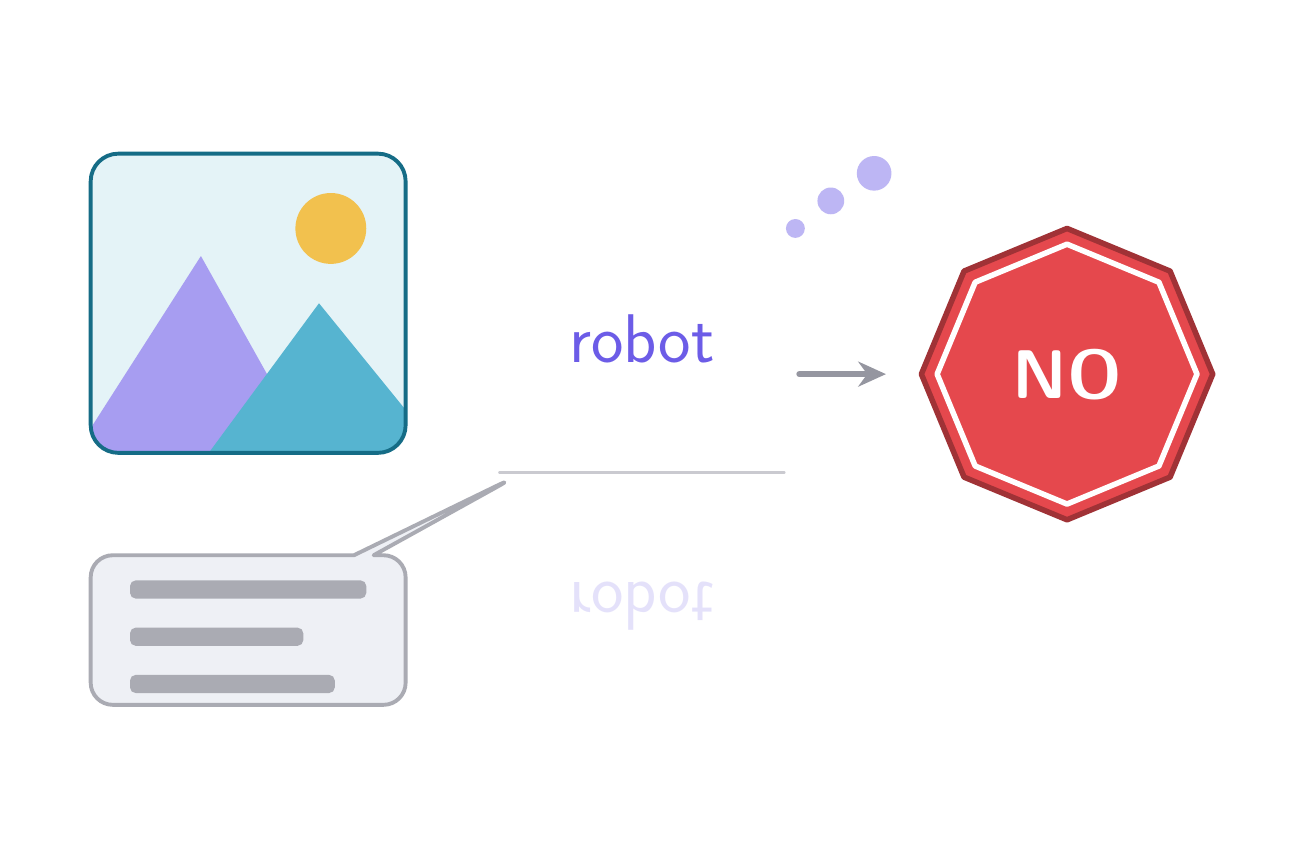
\begin{tikzpicture}
\thumbcanvas
% Visual input.
\begin{scope}
  \clip[rounded corners=10pt] (0.8,4.6) rectangle (4.8,8.4);
  \fill[teal!12] (0.8,4.6) rectangle (4.8,8.4);
  \fill[violet!60] (0.6,4.6) -- (2.2,7.1) -- (3.6,4.6) -- cycle;
  \fill[teal!75] (2.3,4.6) -- (3.7,6.5) -- (5.0,4.9) -- (5.0,4.6) -- cycle;
  \fill[sun] (3.85,7.45) circle (0.45);
\end{scope}
\draw[teal!70!black, line width=1.4pt, rounded corners=10pt] (0.8,4.6) rectangle (4.8,8.4);
% Instruction.
\node[rectangle callout, callout absolute pointer={(6.2,4.3)}, fill=mist, draw=ink!40, line width=1.4pt,
  rounded corners=8pt, minimum width=4cm, minimum height=1.9cm] at (2.8,2.35) {};
\fill[ink!40, rounded corners=2pt] (1.3,2.75) rectangle (4.3,2.98);
\fill[ink!40, rounded corners=2pt] (1.3,2.15) rectangle (3.5,2.38);
\fill[ink!40, rounded corners=2pt] (1.3,1.55) rectangle (3.9,1.78);
% The agent and its reflection.
\node[text=violet] at (7.8,6.05) {\icon[78]{robot}};
\draw[ink!25, line width=1.4pt] (6.0,4.35) -- (9.6,4.35);
\begin{scope}[shift={(7.8,2.65)}, yscale=-1]
  \node[transform shape, text=violet, opacity=0.18] at (0,0) {\icon[78]{robot}};
\end{scope}
\fill[violet!45] (9.75,7.45) circle (0.12) (10.2,7.8) circle (0.17) (10.75,8.15) circle (0.22);
% Saying no.
\draw[arrow=ink!50] (9.8,5.6) -- (10.9,5.6);
\node[regular polygon, regular polygon sides=8, shape border rotate=22.5, fill=alert, draw=alert!70!black,
  line width=2pt, minimum size=3.7cm] at (13.2,5.6) {};
\node[regular polygon, regular polygon sides=8, shape border rotate=22.5, draw=white, line width=2pt,
  minimum size=3.3cm, text=white] at (13.2,5.6) {\fontsize{38}{38}\selectfont\bfseries NO};
\end{tikzpicture}
\end{document}
